\chapter{COVERAGE COLLECTION AND MANAGEMENT}
\label{chap:coverage}

\section{INTRODUCTION}
Functional coverage management for SOC designs presents a number of requirements not always found at lower levels of the design hierarchy. The coverage model for an SOC is typically a filtered union of all models defined by imported IPs combined with additional coverage terms defined by the SOC team. As such, the number of coverage terms in the SOC model tends to be large in comparison to any individual IP. So, there is an intense need to generate and manage the coverage information. The ~\figurename~{\ref{fig:verif_flow.png}} shows how coverage is generated, merged and stored in a database during the verification.
\vspace{15pt}
\begin{figure}[h!]
\centering
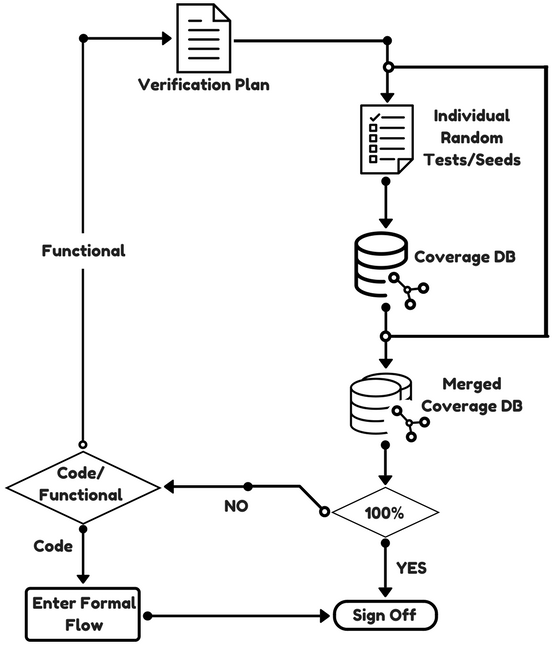
\includegraphics[scale=0.8]{./figures/verif_flow.png}
\caption{Verification Flow}
\label{fig:verif_flow.png}
\end{figure}

\section{COVERAGE COLLECTION FLOW}
After every simulation in a regression, an XML file containing all coverage information for that simulation is generated and copied into a repository unique to that regression. Periodically during the regression, the simulation coverage information residing in the repository is aggregated into a summary coverage XML file. At the end of the regression, only the summary coverage XML file is uploaded. Individual simulation XML coverage results are discarded.
\vspace{15pt}
\begin{figure}[h!]
\centering
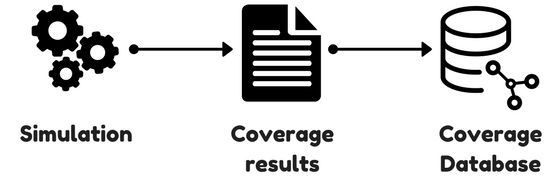
\includegraphics[scale=0.8]{./figures/coverage_collection.png}
\caption{Coverage Collection Flow}
\label{fig:coverage_collection.png}
\end{figure}

\vspace{15pt}
\begin{figure}[h!]
\centering
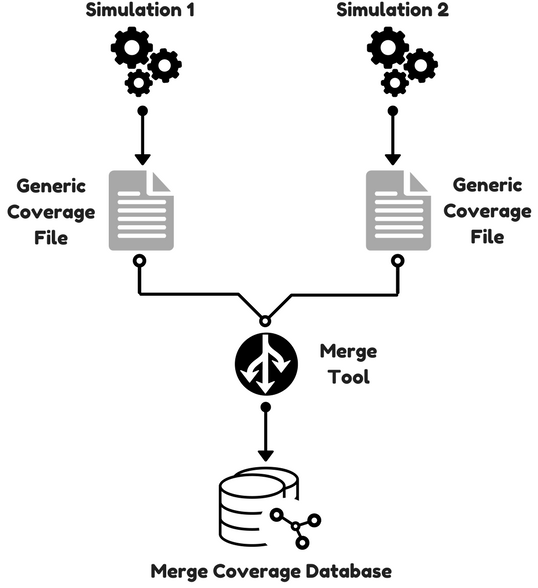
\includegraphics[scale=0.8]{./figures/coverage_management.png}
\caption{Coverage Management Flow}
\label{fig:coverage_management.png}
\end{figure}

\section{EXAMPLE COVERAGE COLLECTION}
Functional coverage model is specified using SystemVerilog. Usually the coverage results are collected by the simulator tools and are dumped in some internal binary format. This example uses \emph{VCS simulator from Synopsys} to illustrate the coverage generation from a testbench. VCS simulation of the testbench generates the coverage and these coverage results are stored in \emph{simv.vdb} directory.

\subsection{TESTBENCH EXAMPLE}
%%\lstinputlisting[language=Verilog]{rtl.sv}
\begin{lstlisting}
module simple_coverage();

logic [7:0]  addr;
logic [7:0]  data;
logic        par;
logic        rw;
logic        en;

covergroup memory @ (posedge en);
  address : coverpoint addr {
    bins low    = {0,50};
    bins med    = {51,150};
    bins high   = {151,255};
  }
  parity : coverpoint  par {
    bins even  = {0};
    bins odd   = {1};
  }
  read_write : coverpoint rw {
    bins  read  = {0};
    bins  write = {1};
  }
endgroup

memory mem = new();

task drive (input [7:0] a, input [7:0] d, input r);
  #5 en <= 1;
  addr  <= a;
  rw    <= r;
  data  <= d;
  par   <= ^d;
  $display ("@%2tns Address :%d data %x, rw %x, parity %x",$time,a,d,r, ^d);
  #5 en <= 0;
  rw    <= 0;
  data  <= 0;
  par   <= 0;
  addr  <= 0;
  rw    <= 0;
endtask

initial begin
  en = 0;
  repeat (10) begin
    drive ($random,$random,$random);
  end
  #10 $finish;
end

endmodule

\end{lstlisting}

\section{SIMULATION OUTPUT}
\begin{verbatim}
@ 5ns Address : 36 data 81, rw 1, parity 0
@15ns Address : 99 data 0d, rw 1, parity 1
@25ns Address :101 data 12, rw 1, parity 0
@35ns Address : 13 data 76, rw 1, parity 1
@45ns Address :237 data 8c, rw 1, parity 1
@55ns Address :198 data c5, rw 0, parity 0
@65ns Address :229 data 77, rw 0, parity 0
@75ns Address :143 data f2, rw 0, parity 1
@85ns Address :232 data c5, rw 0, parity 0
@95ns Address :189 data 2d, rw 1, parity 0

\end{verbatim} 

\section{COVERAGE REPORT}
Simulation of the testbench using VCS simulator generates \emph{simv.vdb} which is the \emph{Verification Database directory}. VCS writes intermediate files and reports about coverage in the form of XML files in subdirectories within in this directory.

To view the coverage report, a reporter utility of VCS named \emph{'urg'} is used.
\vspace{15pt}
\begin{figure}[h!]
\centering
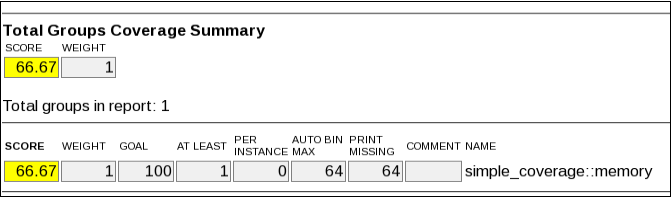
\includegraphics[scale=0.85]{./figures/urgreport2.png}
%\caption{}
\label{fig:urgreport2.png}
\end{figure}

%\vspace{15pt}
\begin{figure}[h!]
\centering
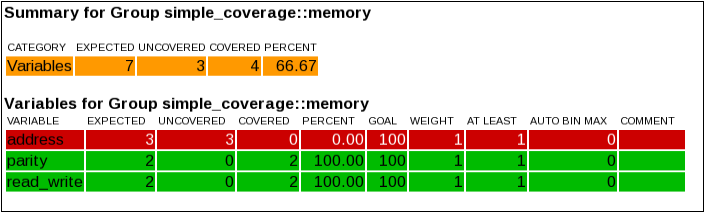
\includegraphics[scale=0.85]{./figures/urgreport3.png}
%\caption{}
\label{fig:urgreport3.png}
\end{figure}

%\vspace{15pt}
\begin{figure}[h!]
\centering
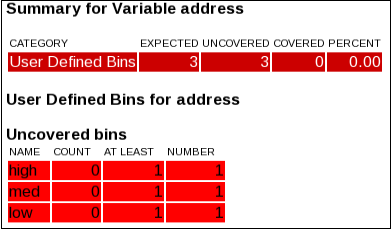
\includegraphics{./figures/urgreport4.png}
%\caption{}
\label{fig:urgreport4.png}
\end{figure}

%\vspace{15pt}
\begin{figure}[h!]
\centering
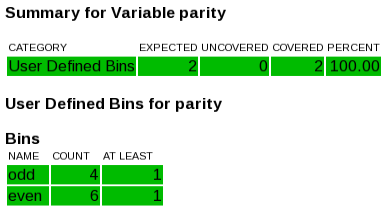
\includegraphics{./figures/urgreport5.png}
%\caption{}
\label{fig:urgreport5.png}
\end{figure}

%\vspace{15pt}
\begin{figure}[h!]
\centering
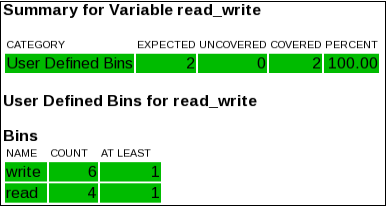
\includegraphics{./figures/urgreport6.png}
%\caption{}
\label{fig:urgreport6.png}
\end{figure}
